% !TEX encoding = UTF-8 Unicode
\documentclass{article}
\usepackage{superstyle}
\begin{document}




\begin{titlepage}

\newcommand{\HRule}{\rule{\linewidth}{0.5mm}} 

\center 

\textsc{\LARGE Matematikk prosjekt 1}\\[1.5cm] % Name of your university/college
\textsc{\Large }\\[0.5cm] % Major heading such as course name
\textsc{\large TDAT2002-A 14H}\\[0.5cm] % Minor heading such as course title

\HRule \\[0.4cm]
{ \huge \bfseries The Euler-Bernoulli beam}\\[0.4cm] 
\HRule \\[1.5cm]


\begin{minipage}{0.4\textwidth}
\begin{flushleft} \large
\emph{Authors:}\\
Lars \textsc{Garberg} \\
Bjørn \textsc{Hoxmark} \\
Borgar \textsc{Lie} \\
Jørgen \textsc{Wilhelmsen}

\end{flushleft}
\end{minipage}
~
\begin{minipage}{0.4\textwidth}
\begin{flushright} \large
\emph{Supervisor:} \\
 Hans Jakob \textsc{Rivertz} % Supervisor's Name
\end{flushright}
\end{minipage}\\[4cm]

% If you don't want a supervisor, uncomment the two lines below and remove the section above
%\Large \emph{Author:}\\
%John \textsc{Smith}\\[3cm] % Your name

%----------------------------------------------------------------------------------------
%	DATE SECTION
%----------------------------------------------------------------------------------------

{\large \today}\\[3cm] % Date, change the \today to a set date if you want to be precise

%----------------------------------------------------------------------------------------
%	LOGO SECTION
%----------------------------------------------------------------------------------------

%\includegraphics{Logo}\\[1cm] % Include a department/university logo - this will require the graphicx package
 
%----------------------------------------------------------------------------------------

\vfill % Fill the rest of the page with whitespace

\end{titlepage}

\newpage


\section{Forord} % (fold)
\label{sec:forord}
Denne rapporten er resultatet av et prosjekt ved dataingeniørlinjen på HiST. Oppgaven har blitt utført vårsemesteret 2015. 
\vspace{5mm}


I vårt arbeid med denne oppgaven har vi benyttet oss av mange teknologier som har forenklet prosessen betraktelig, eksempelvis og spesielt Latex, Github, Google Docs, MatLab og Sublime har alle vært til stor hjelp får å produsere det endelige resultatet. 
\vspace{5mm}

Vi vil også takke Hans Jakob Rivertz for god veiledning gjennom hele prosjektet. 

\newpage
% section forord (end)



\section{Sammendrag} % (fold)
\label{sec:sammendrag}

Denne rapporten tar for seg GPS-problemet (Global Positioning System). GPS er et system bestående av en rekke satelitter som ved hjelp av avstander og tidsforskjeller kan regne ut posisjonen til brukere over hele jordkloden. Da GPS først ble tatt ibruk revolusjonerte det hvordan mennesker generelt kunne lokalisere seg. Idag er GPS er et system som er i ekstremt mye bruk, og man finner det implementert i for eksempel smarttelefoner, bærbare datamaskiner og klokker. Ved å innføre en fjerde satelitts posisjon, kan vi eliminere det originale tidsproblemet for å finne en meget nøyaktig posisjon, i tillegg til den synkroniserte tiden til satelittklokkene. \\

I rapporten går vi først igjennom grunnleggende teori som ligger til utregningene gjort i oppgavene. Vi tar utgangspunkt i formlene boka oppgir, og løser GPS-problemet på bakgrunn av disse. \\

Etter teoridelen løser vi en rekke oppgaver knyttet til GPS-problemet og dets nøyaktighet. Oppgavene går fra å finne forskjellige løsninger på det originale likningssystemet, implementere disse i MatLab, i tillegg til å regne og utføre eksperimenter på hvor nøyaktige resultatene er. Vi viser også hvordan satelittenes posisjon har en påvirkning på det endelige resultatet. 
\newpage
% section sammendrag (end)


%\section{Innholdsfortegnelse og figur- og tabelliste} % (fold)
\label{sec:innholdsfortegnelse_og_figur_og_tabelliste}
\renewcommand{\contentsname}{Innholdsfortegnelse og figur- og tabelliste}
\tableofcontents
\newpage
% section innholdsfortegnelse_og_figur_og_tabelliste (end)



\section{Teori og metode} % (fold)
\label{sec:teori}
GPS' oppgave er å gi mottakeren mest mulig \textit{nøyaktige} koordinater. For å få koordinater med høyst mulig nøyaktighet, finnes tre teknikker som kan resultere i centimeter- og til og med milimeter nøyaktige koordinater: \cite{StrangBorre}
\begin{itemize}
  \item \textbf{Differential Global Positioning System (DGPS).} Denne teknikken går ut på at man har basestasjoner på jorden, der  den nøyaktige posisjonen er kjent. Basestasjonen mottar likevel sin posisjon fra satelitter, og sammenligner denne posisjonen med den riktige. Basestasjonen finner da den feilen som satelittene gir. Når en annen mottaker (med ukjent posisjon) så mottar sin posisjonen fra satelittene, mottar den også feilen som basestasjonen har funnet. Denne feilen legges til i den mottatte posisjonen fra satelittene og mottakeren får dermed en mer nøyaktig posisjon. \cite{DGPS}
  \item \textbf{Repetering av målinger.} Hvis en mottaker mottar flere målinger etter hverandre fra satelittene, vil variansen til alle målingene bli mindre enn bare en måling. Dette vil videre gi en mer nøyaktig posisjon. 
  \item \textbf{Estimering av feil fra alle kilder i hver måling.}  Om man finner feilestimat fra alle mulige kilder og regner med disse i utregningen av posisjonen hos mottakeren, vil nøyaktigheten av posisjonen øke. 
\end{itemize}
Det er det siste punktet dette prosjektet tar for seg. Med hovedvekt på feilestimat i satelittklokkene og hvor tett satelittene er posisjonert. 



%Tre teknikker for å få centimeter- og til og med milimeter nøyaktige posisjoner: [Strang and Borre (1997)]. 
%	- Bruk to eller flere mottakere. Minst en mottaker (basestasjon) har en kjent posisjon, den mottar en "kalkulert posisjon" fra satelitten, og rekner da ut forskjellen mellom sin posisjon og posisjonen den fikk fra satelitten. Når en annen mottaker med ukjent posisjon nå mottar en posisjon fra satelitten, mottar den også feilmarginen fra basestasjonen. Den kan dermed rekne ut sin korrekte posisjon. Dette kalles DGPS. 
%	- Repetering av målinger. Hvis en mottaker mottar flere målinger av sin posisjon etter hverandre, vil variansen til alle målingene bli mindre enn bare en måling. 
%	- Estimere hver feil fra alle kilder i hver måling (klokkeforskjell, forskjellig lyshastighet, tette satelitter osv). 
%	Vi skal i dette prosjektet rekne på det siste punktet.

	% Ê - Ê
	% Þ - Þ
	% å - å
	
% HUSK REFERANSE På DGPS. 
\clearpage

\newpage
% section teori (end)




\section{Resultater} % (fold)
\label{sec:resultater}


\subsection{Oppgave 1} % (fold)
\label{sub:oppgave_1}
%oppgavetekst
	Write a Matlab program to carry out the solution via the quadratic formula. Hint: Subtracting the last three equations of (4.37) from the first yields three linear equations in the four unknowns $x{\vec u_x} + y{\vec u_y} + z{\vec u_z} + d{\vec u_d} + \vec{w} = 0$, expressed in vector form. A formula for x in terms of d can be obtained from 
\begin{align}
0 = det[{\vec u_y}|{\vec u_z}|{\vec u_x} + y{\vec u_y} + z{\vec u_z} + d{\vec u_d} + \vec{w}] \nonumber
\end{align}
noting that the determinant is linear in its columns and that a matrix with a repeated column has determinant zero. Similarly, we can arrive at formulas for y and z, respectively, in terms of d, that can be substituted in the first quadratic equation of (4.37), to make it an equation in one variable. \\ \\

% Her starter oppgavel�sningen. 
\textbf{Løsning:} \\

	I oppgaveteksten blir følgende likningssystem - som er en omskrivning av likningssettet (4.37) omtalt i oppgave 2 - gitt: 
\begin{align}
{(x - {A_1})^2} + {(y - {B_1})^2} + {(z - {C_1})^2} &= {[c({t_1} - d)]^2} \nonumber \\ 
{(x - {A_2})^2} + {(y - {B_2})^2} + {(z - {C_2})^2} &= {[c({t_2} - d)]^2}  \nonumber \\
{(x - {A_3})^2} + {(y - {B_3})^2} + {(z - {C_3})^2} &= {[c({t_3} - d)]^2}  \nonumber \\
{(x - {A_4})^2} + {(y - {B_4})^2} + {(z - {C_4})^2} &= {[c({t_4} - d)]^2} \label{Ex1:system} 
\end{align}

Det er ønskelig løse dette likningssystemet slik at alle x, y, og z er uttrykt med d, slik at det kan lages kvadratiske likninger i form av d, for så å løse dem med hensyn til d. I oppgaveteksten ble det fortalt at om man subtraherer de tre siste likningene fra den første i (\ref{Ex1:system}), vil man få tre linneære likninger. Vi starter med å subtrahere den andre likningen med den første. 

\begin{multline}
{(x - {A_1})^2} - {(x - {A_2})^2} + {(y - {B_1})^2} - {(y - {B_2})^2} + {(z - {C_1})^2} - {(z - {C_2})^2} = 
{[c({t_1} - d)]^2} - {[c({t_2} - d)]^2}  \label{Ex1:linearEqs}
\end{multline}

Vi løser opp andregradsuttrykkene i (\ref{Ex1:linearEqs}) og setter uttrykket lik 0.
\begin{multline}
\\
({x^2} - 2{A_1}x + A_1^2) - ({x^2} - 2{A_2}x + A_2^2)  \\
+ \\
({y^2} - 2{B_1}y + B_1^2) - ({y^2} - 2{B_2}y + B_2^2) \\
+ \\
({z^2} - 2{C_1}z + C_1^2) - ({z^2} - 2{C_2}z + C_2^2)\\
- \\
({c^2}{t_1} - 2{t_1}{c^2} + {c^2}{d^2}) + ({c^2}{t_2} - 2{t_2}{c^2} + {c^2}{d^2}) \\
= \\
0 \\ \nonumber
\end{multline} 

Vi samler så utrykkene slik at x, y og z er samlet, mens de resterende konstantene blir samlet i en variabel kalt \\ $W = {A_1}^2 - {A_2}^2 + {B_1}^2 - {B_2}^2 + {C_1}^2 - {C_2}^2 + ({c^2}( - {t_1}^2 + {t_2}^2))$:  
\begin{multline}
- 2x({A_1} - {A_2}) - 2y({B_1} - {B_2}) - 2z({C_1} - {C_2}) + 2d{c^2}({t_1} - {t_2}) + W = 0
\end{multline}

Merk at likning nr. 3 og 4 også skulle trekkes fra den første fra ligninssettet gitt i (\ref{Ex1:system}). De to nye likningene vil gi de samme resultatene. De eneste forskjellene vil være koordinatene til satelittene. De tre likningene blir:
\begin{align}
- 2x({A_1} - {A_2}) - 2y({B_1} - {B_2}) - 2z({C_1} - {C_2}) + 2d{c^2}({t_1} - {t_2}) + W_1 &= 0 \nonumber \\
- 2x({A_1} - {A_3}) - 2y({B_1} - {B_3}) - 2z({C_1} - {C_3}) + 2d{c^2}({t_1} - {t_3}) + W_2 &= 0  \nonumber\\
- 2x({A_1} - {A_4}) - 2y({B_1} - {B_4}) - 2z({C_1} - {C_4}) + 2d{c^2}({t_1} - {t_4}) + W_3 &= 0 \nonumber \\ \label{Ex1:3equations}
\end{align}

Likningene blir så samlet slik at x-, y-, z-, og d-punktene blir samlet i hver sin vektor. Vektorene uttrykkes ved ${\vec u_x}, {\vec u_y}, {\vec u_z}$ og  ${\vec u_d}$, samt $\vec{w}$. 
\begin{align}
	{\vec u_x} &=  - 2\cdot[{A_1} - {A_2}, \enspace {A_1} - {A_3},  \enspace{A_1} - {A_4}]^T \nonumber \\
	{\vec u_y} &=  - 2\cdot[{B_1} - {B_2},  \enspace{B_1} - {B_3},  \enspace{B_1} - {B_4}]^T \nonumber \\
	{\vec u_z} &=  - 2\cdot[{C_1} - {C_2},  \enspace{C_1} - {C_3},  \enspace{C_1} - {C_4}]^T \nonumber \\
	{\vec u_d} &=  2c^2\cdot[{t_1} - {t_2},  \enspace{t_1} - {t_3},  \enspace{t_1} - {t_4}]^T \nonumber \\
	{\vec w}  &= 
	\begin{bmatrix}
		&{A_1}^2 - {A_2}^2 + {B_1}^2 - {B_2}^2 + {C_1}^2 - {C_2}^2 + ({c^2}( - {t_1}^2 + {t_2}^2)) \\
		&{A_1}^2 - {A_3}^2 + {B_1}^2 - {B_3}^2 + {C_1}^2 - {C_3}^2 + ({c^2}( - {t_1}^2 + {t_3}^2)) \\ 
		&{A_1}^2 - {A_4}^2 + {B_1}^2 - {B_4}^2 + {C_1}^2 - {C_4}^2 + ({c^2}( - {t_1}^2 + {t_4}^2))
	\end{bmatrix}\nonumber \\ \nonumber
\end{align}

Dette er skrevet i MatLab koden på følgende måte: 

\begin{lstlisting}
% Definerer Ux, Uy og Uz som regnet ut i teorien 
Ux = -2 *[A1 - A2; A1 - A3; A1 - A4];
Uy = -2 *[B1 - B2; B1 - B3; B1 - B4];
Uz = -2 *[C1 - C2; C1 - C3; C1 - C4];
Ud = 2 *(c^2)*[t1 - t2; t1 - t3; t1 - t4];
W = [A1^2 - A2^2 + B1^2 - B2^2 + C1^2 - C2^2 - (c^2)*(t1^2) + (c^2)*(t2^2); 
     A1^2 - A3^2 + B1^2 - B3^2 + C1^2 - C3^2 - (c^2)*(t1^2) + (c^2)*(t3^2); 
     A1^2 - A4^2 + B1^2 - B4^2 + C1^2 - C4^2 - (c^2)*(t1^2) + (c^2)*(t4^2)]; 
\end{lstlisting}

Vi får da uttrykket $x\cdot{\vec u_x} + y\cdot{\vec u_y} + z\cdot{\vec u_z} + d\cdot{\vec u_d} + {\vec w} = 0$. \newpage

%jorgen kommer her 

I boken står det at vi kan komme frem til en formel for x, uttrykt ved d, fra uttrykket $0=\text{det}[\vec{u}_y | \vec{u}_z | x\vec{u}_x + y\vec{u}_y + z\vec{u}_z + d\vec{u}_d + \vec{w}]$. Vi setter opp vektoren: 

\begin{align} \label{eq:detx}
	\text{det}[\vec{u}_y|\vec{u}_z |x\vec{u}_x + y\vec{u}_y + z\vec{u}_z + d\vec{u}_d + \vec{w}]=0
\end{align}

Vi ønsker å utlede et uttrykk for x fra denne determinanten. Determinanten for matrisen i likning \ref{eq:detx} kan skrives om på følgende måte \cite{TheDeterminant}: 

\begin{align}
	&\text{det}[\vec{u}_y|\vec{u}_z | x\vec{u}_x] \nonumber
	\\+ &\text{det}[\vec{u}_y|\vec{u}_z | y\vec{u}_y] \nonumber
	\\+ &\text{det}[\vec{u}_y|\vec{u}_z | z\vec{u}_z] \nonumber
	 \\+&\text{det}[\vec{u}_y|\vec{u}_z | d\vec{u}_d] \nonumber
	\\+ &\text{det}[\vec{u}_y|\vec{u}_z | \vec{w}]\nonumber
	\\&=0
\end{align}
%double end

Videre bruker vi loven som sier at matriser med repeterende kolonner er 0\cite{Determinants}. Da står vi igjen med: 

\begin{align} \label{eq:det_final}
	\text{det}[\vec{u}_y|\vec{u}_z | x\vec{u}_x] 
	+ \text{det}[\vec{u}_y|\vec{u}_z | d\vec{u}_d] 
	+ \text{det}[\vec{u}_y|\vec{u}_z | \vec{w}]
	=0
\end{align}

Den første delen av determinanten uttrykt i likning \ref{eq:det_final} kan løses opp og få x på utsiden \cite{TheDeterminant}. Det samme kan gjøres hvor d inngår i matrisen. Da står vi igjen med: 

\begin{align}
	x\cdot\text{det}[\vec{u}_y|\vec{u}_z | \vec{u}_x] 
	+ d\cdot\text{det}[\vec{u}_y|\vec{u}_z | \vec{u}_d] 
	+ \text{det}[\vec{u}_y|\vec{u}_z | \vec{w}]
	=0 \nonumber 
	\\ 
	x\cdot\text{det}[\vec{u}_y|\vec{u}_z | \vec{u}_x] 
	= -d\cdot\text{det}[\vec{u}_y|\vec{u}_z | \vec{u}_d] 
	-\text{det}[\vec{u}_y|\vec{u}_z | \vec{w}]\nonumber 
\end{align}
Til slutt setter vi x alene. Da står vi igjen med: 

\begin{align}
    x=\frac{-d\cdot\text{det}[\vec{u}_y|\vec{u}_z | \vec{u}_d] 
	-\text{det}[\vec{u}_y|\vec{u}_z | \vec{w}]}{\text{det}[\vec{u}_y|\vec{u}_z | \vec{u}_x]}
\end{align}

For å finne uttrykk for henholdsvis y og z bruker vi samme metode, men med forskjellige utgangsvektorer. På grunn av at en matrise som inneholder lineært avhengige vektorer har determinant = 0 \cite{Determinants}, kan vi sette opp likninger for dette. Ved å veksle mellom å sette inn $\vec{u}_x$, $\vec{u}_y$ og $\vec{u}_z$ som de to første vektorene får vi gunstige startmatriser vi kan bruke for å uttrykke x, y og z med d. For y har vi følgende vektor som start: 

\begin{align} \label{eq:dety}
	\text{det}[\vec{u}_x|\vec{u}_z |x\vec{u}_x + y\vec{u}_y + z\vec{u}_z + d\vec{u}_d + \vec{w}]=0
\end{align}

For z har vi følgende vektor som start: 
\begin{align} \label{eq:detz}
	\text{det}[\vec{u}_x|\vec{u}_y |x\vec{u}_x + y\vec{u}_y + z\vec{u}_z + d\vec{u}_d + \vec{w}]=0
\end{align}

Bruker vi samme fremgangsmåte som for x, ender vi opp med følgende uttrykk for x, y og z: 

\begin{align}\label{eq:x}
    x=\frac{-d\cdot\text{det}[\vec{u}_y|\vec{u}_z | \vec{u}_d] 
	-\text{det}[\vec{u}_y|\vec{u}_z | \vec{w}]}{\text{det}[\vec{u}_y|\vec{u}_z | \vec{u}_x]}
\end{align}

\begin{align}\label{eq:y}
    y=\frac{-d\cdot\text{det}[\vec{u}_x|\vec{u}_z | \vec{u}_d] 
	-\text{det}[\vec{u}_x|\vec{u}_z | \vec{w}]}{\text{det}[\vec{u}_x|\vec{u}_z | \vec{u}_y]}
\end{align}

\begin{align}\label{eq:z}
    z=\frac{-d\cdot\text{det}[\vec{u}_x|\vec{u}_y | \vec{u}_d] 
	-\text{det}[\vec{u}_x|\vec{u}_y | \vec{w}]}{\text{det}[\vec{u}_x|\vec{u}_y | \vec{u}_z]}
\end{align}

Nå har vi altså fått uttrykt både x, y og z ved d. Vi kunne her ha uttrykt uttrykkene med den samme nevneren, ved å bruke loven som sier at vi kan endre fortegn til en determinant så lenge vi bytter plass på 2 rader \cite{TheDeterminant}. For nå å gå videre, setter vi disse inn i bokas likning 4.38. Dette vil resultere i en likning som inneholder d i første og andre grad, og vi kan derav finne d ved å bruke andregradsformelen. Med andre ord vil vi få ett utrykk som vi kan skrive som $Ad^2+Bd+C=0$ Andregradsformelen er gitt ved $d=\frac{-B \pm \sqrt{B^2-4AC}}{2A}$. Før vi setter uttrykkene vi har funnet for x, y og z inn i bokas likning 4.38, deler vi de opp i flere variabler for å gjøre uttrykket ryddigere. Vi setter

\begin{align}
	x_1&=\frac{-d\cdot\text{det}[\vec{u}_y|\vec{u}_z | \vec{u}_d]}{\text{det}[\vec{u}_y|\vec{u}_z | \vec{u}_x]}\nonumber 
\end{align}

\begin{align}
	x_2&=\frac{-d\cdot\text{det}[\vec{u}_y|\vec{u}_z | \vec{w}]}{\text{det}[\vec{u}_y|\vec{u}_z | \vec{u}_x]}\nonumber 
\end{align}

\begin{align}
	y_1&=\frac{-d\cdot\text{det}[\vec{u}_x|\vec{u}_z | \vec{u}_d]}{\text{det}[\vec{u}_x|\vec{u}_z | \vec{u}_y]}\nonumber 
\end{align}

\begin{align}
    y_2&=\frac{-d\cdot\text{det}[\vec{u}_x|\vec{u}_z | \vec{w}]}{\text{det}[\vec{u}_x|\vec{u}_z | \vec{u}_y]}\nonumber 
\end{align}

\begin{align}
    z_1&=\frac{-d\cdot\text{det}[\vec{u}_x|\vec{u}_y | \vec{u}_d]}{\text{det}[\vec{u}_x|\vec{u}_y | \vec{u}_z]}\nonumber
\end{align}

\begin{align}
    z_2&=\frac{-d\cdot\text{det}[\vec{u}_x|\vec{u}_y | \vec{w}]}{\text{det}[\vec{u}_x|\vec{u}_y | \vec{u}_z]}\nonumber 
\end{align}

I MatLab er dette kodet på følgende måte: 
\begin{lstlisting}
	%Dette bruker vi til å løse andregradslikningen for D. Definerer deler 
	%av uttrykket som forklart i teoridelen 
	x1 = -det([Uy Uz Ud])/det([Uy Uz Ux]);
	x2 = -det([Uy Uz W])/det([Uy Uz Ux]);

	y1 = -det([Ux Uz Ud])/det([Ux Uz Uy]);
	y2 = -det([Ux Uz W])/det([Ux Uz Uy]);

	z1 = -det([Ux Uy Ud])/det([Ux Uy Uz]);
	z2 = -det([Ux Uy W])/det([Ux Uy Uz]);
\end{lstlisting} 

Av dette følger det at $x=x_1+x_2$, $y=y_1+y_2$ og $z=z_1+z_2$. Setter vi nå dette inn i første likningen i bokas likning 4.38 får vi: 
\begin{multline}
	\\
    ((x_1+x_2)-A_1)^2+((y_1+y_2)-B_1)^2+((z_1+z_2)-C_1)^2\\
    =\\
    (c(t_1-d))^2 \\\nonumber
\end{multline}
\begin{multline}
	\\
  (x_1+x_2)^2-2A(x_1+x_2)+A^2+(y_1+y_2)^2-2B(y_1+y_2)+B^2\\
    +\\
    (z_1+z_2)^2-2C(z_1+z_2)+C^2-(c(t_1-d))^2\\
    =0 \nonumber 	\\
\end{multline}
\begin{multline}\label{eq:d_expanded}
    \\
    x_1^2+2x_1x_2+x_2^2-2Ax_1-2Ax_2+A^2+y_1^2+2y_1y_2+y_2^2-2By_1-2By_2+B^2\\
    +\\
    z_1^2+2z_1z_2+z_2^2-2Cz_1-2Cz_2+C^2-c^2t^2-c^22td-c^2d^2 \\
    = 0\\
\end{multline}
Som vi ser i utregning \ref{eq:d_expanded} har vi satt inn uttrykkene vi har funnet for x, y og z. Videre ønsker vi å samle alle leddene som vil få $d^2$ for seg, leddene med $d^1$ for seg og resten i en siste gruppe. Da vi ga verdier til $x_1$, $y_1$ og $z_1$, ser vi at det er bare disse leddene som inneholder en d. Det vil si at de eneste leddene hvor d blir i andre grad, er leddene hvor $x_1$, $y_1$ og $z_1$ er opphøyd i andre. Disse samler vi og setter inn i A i andregradsformelen. Videre vil alle leddene som inneholder d i første grad være der hvor $x_1$, $y_1$ og $z_1$ står i første grad. Disse samler vi i B i andregradsformelen. Vi har altså samlet alle koeffisientene som står foran $d^2$ i A, koeffisientene foran $d^1$ i B mens resten av leddene samles i C. A, B og C blir da som følger: 

\begin{align}
    A&=x_1^2+y_1^2+z_1^2-c^2 \\
    B&=2x_1x_2-2Ax_1+2y_1y_2-2By_1+2z_1z_2-2Cz_1-c^22t\\
    C&=x_2^2-2Ax_2+A^2+y_2^2-2By_2+B^2+z_2^2-2Cz_2+C^2-c^2t^2
\end{align}
Dette setter vi inn i andregradsformelen, og får derav 2 verdier for d. 
\begin{lstlisting}
A = (x1^2 + y1^2 + z1^2 - c^2);
B = 2*((x1*x2 - x1*A1) + (y1*y2 - y1*B2) + (z1*z2 - z1*C1)+ t1*c^2);
C = (x2^2 - 2*A1*x2 + A1^2) + (y2^2 -2*B1*y2 + B1^2) + (z2^2 - 2*C1*z2 + C1^2) - (c^2*t1^2);
dd(1) = (-B + sqrt(B^2 - 4*A*C))/(2*A);
dd(2) = (-B - sqrt(B^2 - 4*A*C))/(2*A);
\end{lstlisting}
Til slutt regner vi ut 2 verdier for x, y og z ved å bruke formlene \ref{eq:x}, \ref{eq:y} og \ref{eq:z}. Måten vi skiller mellom disse på er at vi sjekker om koordinatparene befinner seg omtrent på jordas overflate. Det vil alltid være ett sett av koordinater som ikke gjør det, og vi kan deretter utelukke dette settet. 
I MatLab er dette gjort på følgende måte: 

\begin{lstlisting}
	%Første løsning for x, y og z. Setter inn den ene verdien 
	%funnet d i uttrykket for x, y og z gitt i teorien:
	x = x1*dd(1) + x2;
	y = y1*dd(1) + y2;
	z = z1*dd(1) + z2;

	%Finner de andre verdiene
	xx = x1*dd(2) + x2;
	yy = y1*dd(2) + y2;
	zz = z1*dd(2) + z2;

	svar = [x y z;xx yy zz]; 

	%Finner hvilket sett som befinner seg på jordas overflate
	riktig_pos = 2;
	if (abs(svar(1,3) - 6371) < abs(svar(2,3) - 6371)) riktig_pos = 1; end

	%Setter riktige koordinater
	x= svar(riktig_pos,1); 
	y= svar(riktig_pos,2); 
	z= svar(riktig_pos,3); 
	d=dd(riktig_pos); 
	end
\end{lstlisting}

Resultatet av dette er vist i figur \ref{fig:task2result}. 

\begin{figure}[h]
    \centering
    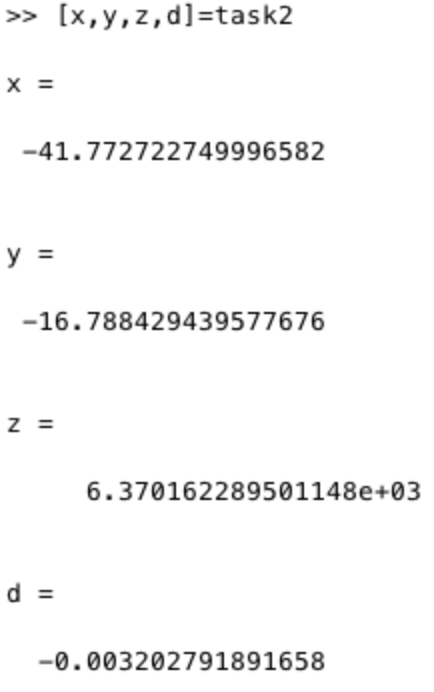
\includegraphics[width=0.4\textwidth]{sections/Exercise1/task2result.png}
    % 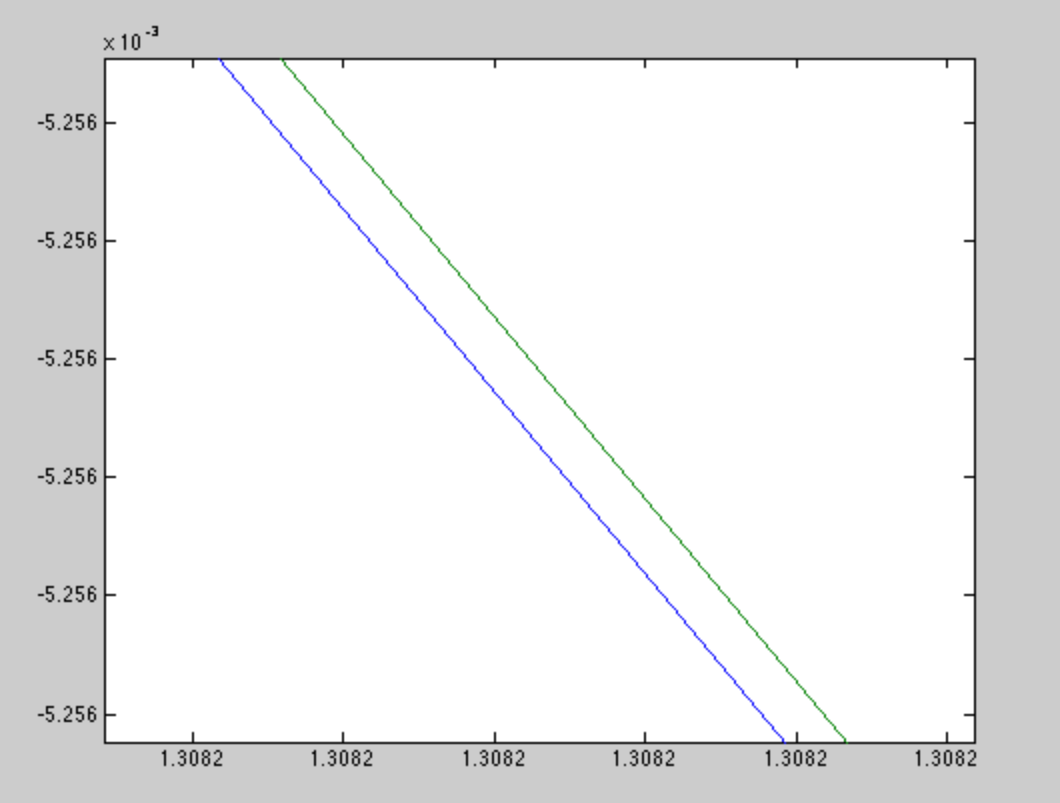
\includegraphics[width=0.4\textwidth]{errorplot2}
    \caption{Task2.m - result}
    \label{fig:task2result}
\end{figure}
\newpage
% subsection oppgave_1 (end)


\subsection{Oppgave 3} % (fold)
\label{sub:oppgave_3}
% !TEX encoding = UTF-8 Unicode
% \documentclass{article}
% \usepackage{../../superstyle}
% \usepackage{listings}
% \usepackage{amsmath}
% \begin{document}
% remove all before

%oppgavetekst
Oppgavetekst

\vspace{5mm}
Løsning

% remove after
% \end{document}
\newpage
% subsection oppgave_3 (end)


\subsection{Oppgave 4} % (fold)
\label{sub:oppgave_4}

Oppgavetekst
Now set up a test of the conditioning of the GPS problem. Define satellite positions $(A_i,B_i,C_i)$ from spherical coordinates $(\rho,\phi i,\theta i)$ as

\begin{align}
	A_i &= \rho \cos{\phi i} \cos{\theta i} \nonumber \\
	B_i &= \rho \cos{\phi i} \sin{\theta i} \nonumber \\
	C_i &= \rho \sin{\theta i} \nonumber \\
\end{align}

where $\rho = 26570$ km is fixed, while $0 \leq \phi_i \leq \frac{\pi}{2}$ and $0 \leq \theta_i \leq 2 \pi$ for $i=1,...,4$ are chosen arbitrarily. The $\phi$ coordinate is restricted so that the four satellites are in the upper hemisphere. Set $x = 0$, $y = 0$, $z = 6370$, $d = 0.0001$, and calculate the corresponding satellite ranges $R_i = \sqrt{A_i^2 + B_i^2 + (C_i − 6370)^2}$ and travel times $t_i = d + R_i /c$.

We will define an error magnification factor specially tailored to the situation. The atomic clocks aboard the satellites are correct up to about 10 nanoseconds, or $10^{−8}$ second. Therefore, it is important to study the effect of changes in the transmission time of this magnitude. Let the backward, or input error be the input change in meters. At the speed of light, $t_i = 10^{−8}$ second corresponds to $10^{−8}c \approx 3$ meters. Let the forward, or output error be the change in position $||(\Delta x,\Delta y,\Delta z)||_\infty$, caused by such a change in $t_i$, also in meters. Then we can define the dimensionless 

\begin{align}
    \text{error magnification factor} = \frac{||(\Delta x,\Delta y,\Delta z)||_\infty}{c||(\Delta t_1,...,\Delta t_m)||_\infty} \nonumber
\end{align}

and the condition number of the problem to be the maximum error magnification factor for all small $\Delta t_i$ (say, $10^{−8}$ or less).

Change each $t_i$ defined in the foregoing by $t_i = +10^{-8}$or $−10^{−8}$, not all the same. Denote the new solution of the equations (4.37) by $(\bar{x},\bar{y},\bar{z},\bar{d})$, and compute the difference in position $||(\Delta x,\Delta y,\Delta z)||_\infty$ and the error magnification factor. Try different variations of the $\Delta t_i$'s. What is the maximum position error found, in meters? Estimate the condition number of the problem, on the basis of the error magnification factors you have computed. 

\textbf{Løsning}

\begin{lstlisting}[caption={task4.m},label=lst:task4.m]
function [conditionNumber, worst_max_pos_error] = task4()
	%definerer konstanter gitt i oppgaven, og lager tilfeldige punkter 
	%phi ogtheta
	rho = 26570;
	c = 299792.458;
	phi = [0.3, 1.2, pi/8, pi/6];
	theta = [1.2,2,3,4.5];

	%Lager vektorer A, B og C, og fyller inn verdiene gitt i oppgaven
	A = ones(1,4); 
	B = ones(1,4); 
	C = ones(1,4);

	for i=1:4
	    A(i) = rho * cos(phi(i)) * cos(theta(i));
	    B(i) = rho * cos(phi(i)) * sin(theta(i));
	    C(i) = rho * sin(phi(i));
	end

	%Lager en R- og t-vektor som definert i teksten
	R = sqrt((A.^2)+(B.^2)+((C-6370).^2));
	t = 0.0001 + (R/c);

	%Lager en riktig løsning, løst ved koden i task2general. 
	[x,y,z,d]= task2general(A,B,C,t); 
	riktig = [x y z d];

	%Definerer en matrise som inneholder alle mulige kombinasjoner av + og - 
	factor = [[-1,-1,-1,1];[-1,-1,1,1];[-1,1,1,1];
			  [-1,1,-1,1];[-1,1,1,-1];[-1,-1,1,-1];
			  [-1,1,-1,-1];[1,1,1,-1];[1,1,-1,-1];
			  [1,-1,-1,-1];[1,-1,1,-1];[1,-1,-1,1];
			  [1,1,-1,1];[1,-1,1,1]];

	max_pos_error = zeros(1,14);
	emf = zeros(1,14);

	%regner ut nye tider basert på faktorene, og løser problemet igjen med
	%task2general. Finner deretter ut den maksimale posisjonsfeilen, samt 
	%EMF for hver utregning.
	for i = 1:length(factor)
	    dt1(1) = t(1) + 1e-8*factor(i,1);
	    dt1(2) = t(2) + 1e-8*factor(i,2);
	    dt1(3) = t(3) + 1e-8*factor(i,3);
	    dt1(4) = t(4) + 1e-8*factor(i,4); 
	    [x2,y2,z2,d2]=task2general(A,B,C,dt1);
	    feil = [x2 y2 z2 d2];
	    max_pos_error(i) = max(abs(riktig-feil));
	    emf(i) = max_pos_error(i)/(c*max(abs(dt1-t)));
	end


	full(max_pos_error)
	full(emf)

	%Finner den største posisjonsfeilen og kondisjonstallet.
	worst_max_pos_error = max(full(max_pos_error));
	conditionNumber = max(emf);

end
\end{lstlisting}

\begin{lstlisting}[caption={task2general.m}]
function [x,y,z,d] = task2general(A, B, C, t)
	A1=A(1); 
	A2=A(2); 
	A3=A(3); 
	A4=A(4); 
	t1=t(1); 

	B1=B(1); 
	B2=B(2); 
	B3=B(3); 
	B4=B(4); 
	t2=t(2); 

	C1=C(1); 
	C2=C(2); 
	C3=C(3); 
	C4=C(4); 
	t3=t(3); 
	t4=t(4);
	%Lyshastigheten c

	c = 299792.458;

	% Definerer Ux, Uy og Uz som regnet ut i teorien 
	Ux = -2 *[A1 - A2; A1 - A3; A1 - A4];
	Uy = -2 *[B1 - B2; B1 - B3; B1 - B4];
	Uz = -2 *[C1 - C2; C1 - C3; C1 - C4];
	Ud = 2 *(c^2)*[t1 - t2; t1 - t3; t1 - t4];
	W = [A1^2 - A2^2 + B1^2 - B2^2 + C1^2 - C2^2 - (c^2)*(t1^2) + (c^2)*(t2^2); 
	     A1^2 - A3^2 + B1^2 - B3^2 + C1^2 - C3^2 - (c^2)*(t1^2) + (c^2)*(t3^2); 
	     A1^2 - A4^2 + B1^2 - B4^2 + C1^2 - C4^2 - (c^2)*(t1^2) + (c^2)*(t4^2)];

	%Dette bruker vi til å løse andregradslikningen for D. Definerer
	%deler av uttrykket som %forklart i teoridelen 
	x1 = -det([Uy Uz Ud])/det([Uy Uz Ux]);
	x2 = -det([Uy Uz W])/det([Uy Uz Ux]);

	y1 = -det([Ux Uz Ud])/det([Ux Uz Uy]);
	y2 = -det([Ux Uz W])/det([Ux Uz Uy]);

	z1 = -det([Ux Uy Ud])/det([Ux Uy Uz]);
	z2 = -det([Ux Uy W])/det([Ux Uy Uz]);

	% Setter opp A, B og C som skal brukes i andregradsformelen. Disse er
	% regnet ut og vist i teorien: 

	A = (x1^2 + y1^2 + z1^2 - c^2);
	B = 2*((x1*x2 - x1*A1) + (y1*y2 - y1*B2) + (z1*z2 - z1*C1)+ t1*c^2);
	C = (x2^2 - 2*A1*x2 + A1^2) + (y2^2 -2*B1*y2 + B1^2) + (z2^2 - 2*C1*z2 + C1^2) - (c^2*t1^2);
	dd(1) = (-B + sqrt(B^2 - 4*A*C))/(2*A);
	dd(2) = (-B - sqrt(B^2 - 4*A*C))/(2*A);

	%Første løsning for x, y og z. Setter inn den ene verdien for d i 
	%uttrykket for x, y og z gitt i teorien:
	x = x1*dd(1) + x2;
	y = y1*dd(1) + y2;
	z = z1*dd(1) + z2;

	%Finner de andre verdiene
	xx = x1*dd(2) + x2;
	yy = y1*dd(2) + y2;
	zz = z1*dd(2) + z2;

	svar = [x y z;xx yy zz]; 

	riktig_pos = 2;
	if (abs(abs(svar(1,3)) - 6371) < abs(abs(svar(2,3)) - 6371)) riktig_pos = 1; end
	x = svar(riktig_pos,1); 
	y = svar(riktig_pos,2); 
	z = svar(riktig_pos,3); 
	d = dd(riktig_pos); 
end
\end{lstlisting}

Alle verdiene for EMF og den maksimale posisjonsfeilen for de 14 forskjellige mulighetene er vist i tabellene \ref{fig:task4EMF} og \ref{fig:task4max_pos_error}. I grafene \ref{fig:task4EMF_graph} og \ref{fig:task4max_pos_error_graph} er utviklingen til disse tallene vist, etterhvert som fortegnene til tillegget på de 4 tidene endrer seg. 

\begin{figure}[h]
	\begin{minipage}{.5\textwidth}
		\centering
		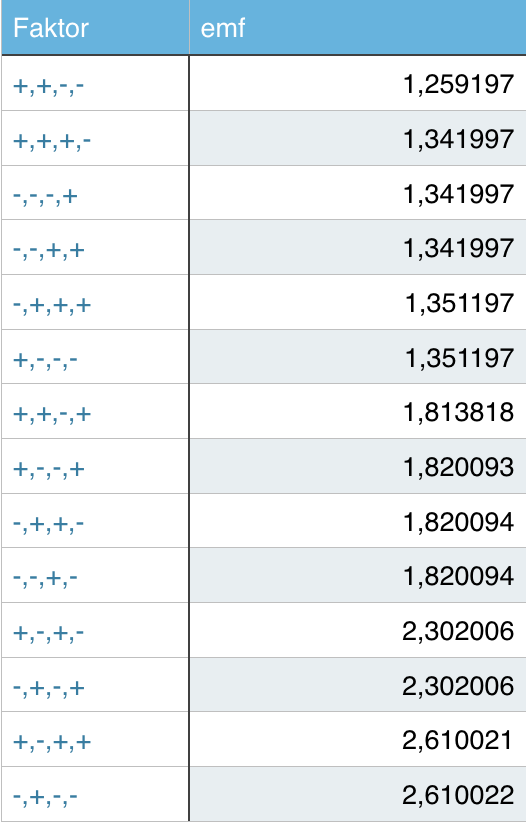
\includegraphics[width=0.8\textwidth]{sections/Exercise4/task4emf.png}
			\caption{Task 4 - EMF tabell}
			\label{fig:task4EMF}
	\end{minipage}
	\vspace{20 mm}
	\begin{minipage}{.5\textwidth}
	Av tabellen og grafen ser vi at de forskjellige kombinasjonene av faktorene tydelig deler seg inn i forskjellige nivåer, hvor kombinasjonene på samme nivå har ca. lik verdi. Kombinasjonene som er motsetninger av hverandre befinner seg på samme nivå. Hvilke kombinasjoner som befinner seg på de forskjellige nivåene avhenger av hvilke satelitter som bidrar med de ulike tidsforskjellene.
	\end{minipage}

	\centering
    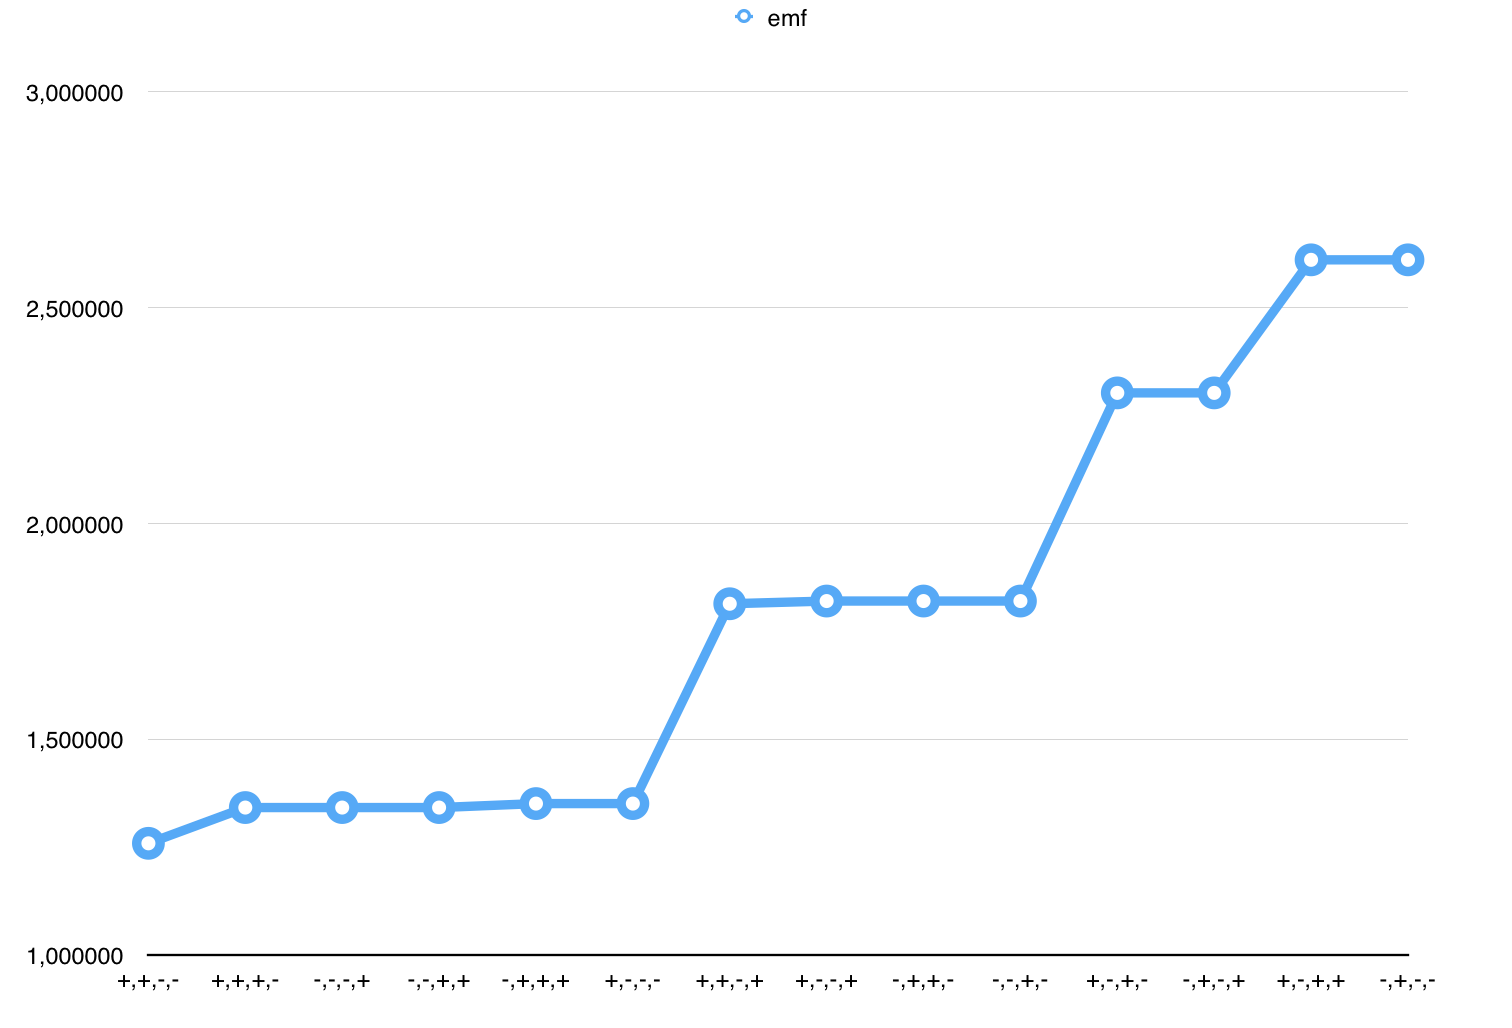
\includegraphics[width=0.8\textwidth]{sections/Exercise4/task4emf_graph.png}
	    \caption{Task 4 - EMF graf}
	    \label{fig:task4EMF_graph}
\end{figure}

\begin{figure}
	\begin{minipage}{.5\textwidth}
		\centering
		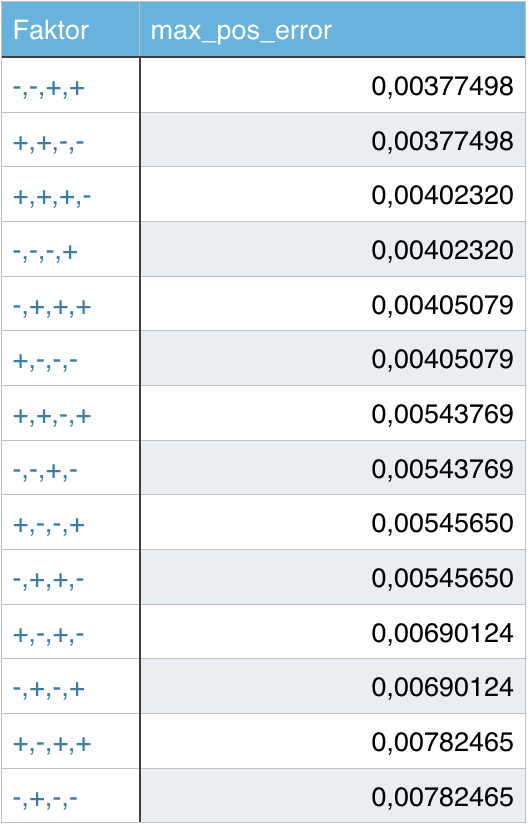
\includegraphics[width=0.8\textwidth]{sections/Exercise4/task4max_pos_error.png}
	    	\caption{Task 4 - Maks. pos. tabell}
	    	\label{fig:task4max_pos_error}
	\end{minipage}
	\vspace{20 mm}
	\begin{minipage}{.5\textwidth}
		Vi ser av tabellen og grafen for den maksimale posisjonsfeilen at verdiene grupperer seg og vokser på samme måte som verdiene for EMF. 
	\end{minipage}

	\centering
	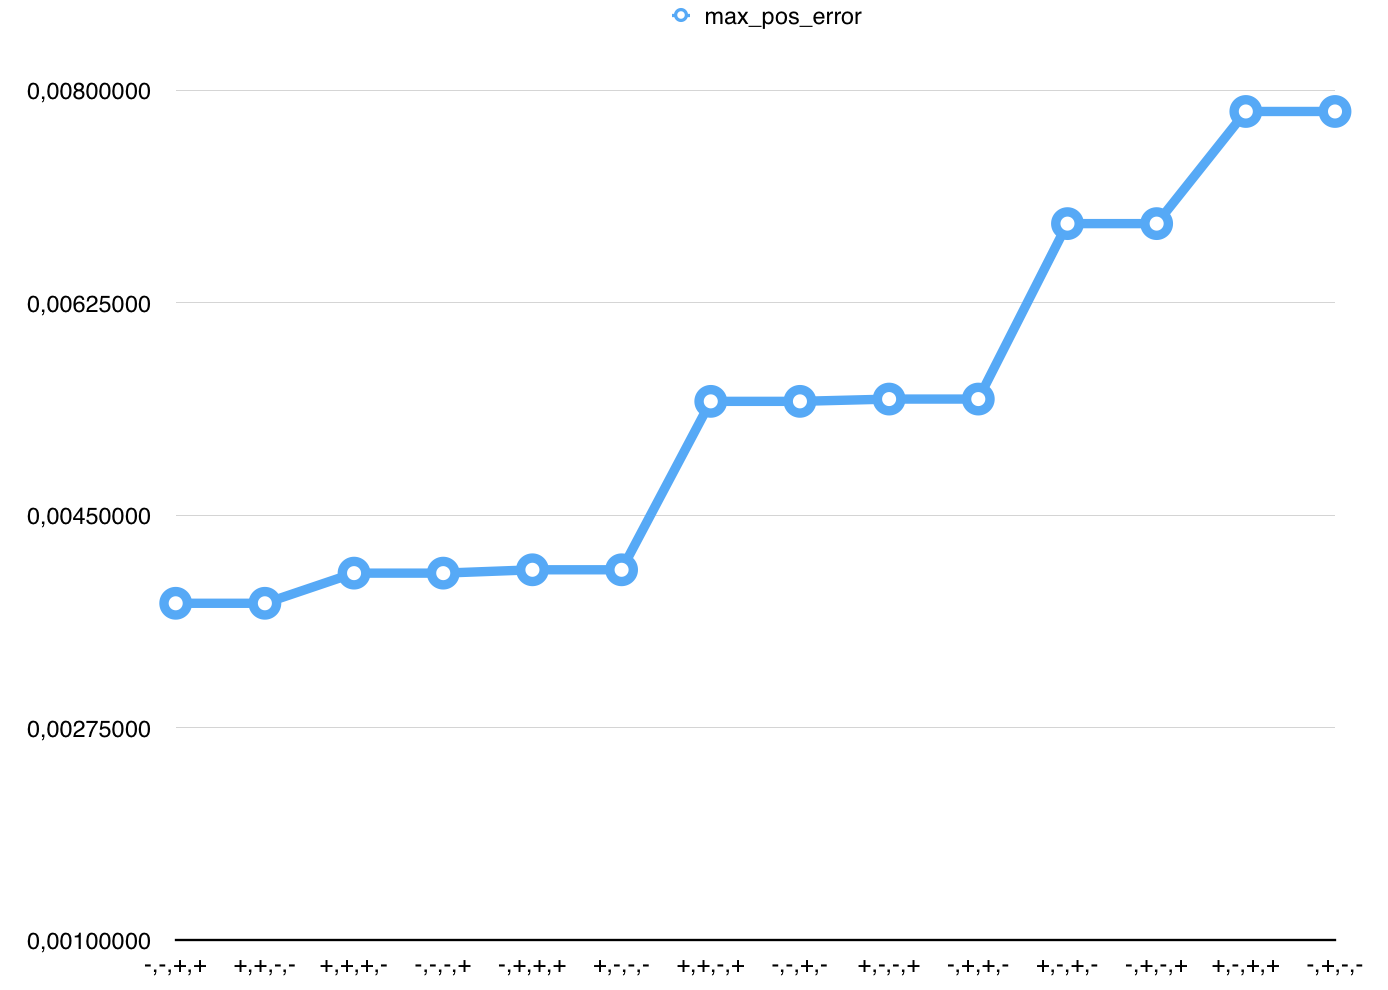
\includegraphics[width=0.8\textwidth]{sections/Exercise4/task4max_pos_error_graph.png}
	    \caption{Task 4 - Maksimal posisjonsfeil graf}
	    \label{fig:task4max_pos_error_graph}
\end{figure}
I figur \ref{fig:task4answer} er de største verdiene for både EMF og den maksimale posisjonsfeilen vist. Dette er det som blir returnert av koden vist i listing \ref{lst:task4.m}. 

\begin{figure}[h]
	\centering
	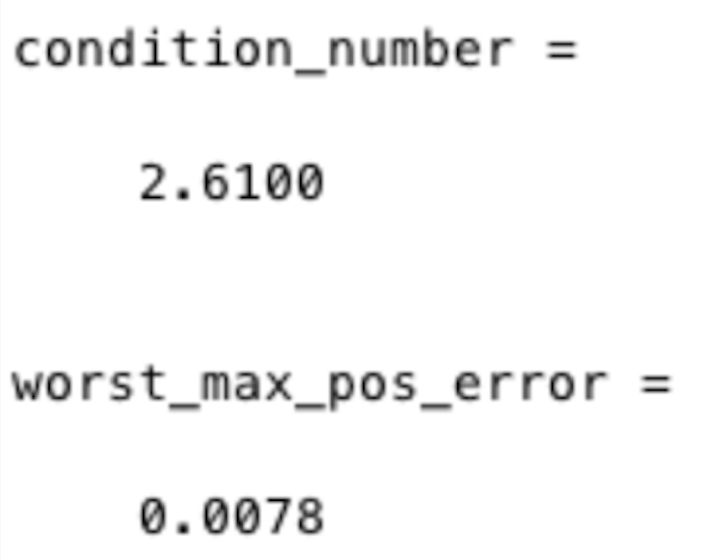
\includegraphics[width=0.4\textwidth]{sections/Exercise4/task4answer.png}
	\caption{Task4.m - resultat}
	\label{fig:task4answer}
\end{figure}
\newpage
% subsection oppgave_4 (end)


\subsection{Oppgave 5} % (fold)
\label{sub:oppgave_5}
% !TEX encoding = UTF-8 Unicode
\documentclass{article}
\usepackage{../../superstyle}
\usepackage{listings}
\usepackage{amsmath}
\begin{document}
% remove all before

%oppgavetekst
Oppgave tekst: 

Now repeat Step 4 with a more tightly grouped set of satellites. Choose all $\phi$$_i$ within
5 percent of one another and all $\theta$$_i$ within 5 percent of one another. Solve with and without the same input error as in Step 4. Find the maximum position error and error magnification factor. Compare the conditioning of the GPS problem when the satellites are tightly or loosely bunched.

\vspace{5mm}
Løsning

\begin{lstlisting}[caption={Task3.m}]
function [conditionNumber, worst_max_pos_error] = task5()

rho = 26570;

phi = [pi/4 (pi/4)*1.015 (pi/4)*1.03 (pi/4)*1.045];
theta = [pi pi*1.015 pi*1.030 pi*1.045];
A = ones(1,4); 
B = ones(1,4); 
C = ones(1,4);

for i=1:4
    A(i) = rho * cos(phi(i)) * cos(theta(i));
    B(i) = rho * cos(phi(i)) * sin(theta(i));
    C(i) = rho * sin(phi(i));
end

c = 299792.458;

R = sqrt((A.^2)+(B.^2)+((C-6370).^2));
t = 0.0001 + (R/c);

[x,y,z,d]= task2general(A,B,C,t); 
riktig = [x y z d];

factor = [[-1,-1,-1,-1];[1,1,1,1];[-1,-1,-1,1];[-1,-1,1,1];
		  [-1,1,1,1];[-1,1,-1,1];[-1,1,1,-1];[-1,-1,1,-1];
		  [-1,1,-1,-1];[1,1,1,-1];[1,1,-1,-1];[1,-1,-1,-1];
		  [1,-1,1,-1];[1,-1,-1,1];[1,1,-1,1];[1,-1,1,1]];

max_pos_error = zeros(1,16);
emf = zeros(1,16);

for i = 1:length(factor)
    dt1(1) = t(1) + 1e-8*factor(i,1);
    dt1(2) = t(2) + 1e-8*factor(i,2);
    dt1(3) = t(3) + 1e-8*factor(i,3);
    dt1(4) = t(4) + 1e-8*factor(i,4); 
    [x2,y2,z2,d2]=task2general(A,B,C,dt1);
    feil = [x2 y2 z2 d2];
    max_pos_error(i) = max(abs(riktig-feil));
    emf(i) = max_pos_error(i)/(c*max(abs(dt1-t)));
end

worst_max_pos_error = max(max_pos_error);
conditionNumber = max(emf);

end
\end{lstlisting}

\begin{figure}[h]
    \centering
    % \includegraphics[width=0.9\textwidth]{sections/Exercise5/task5result}
    \includegraphics[width=0.9\textwidth]{task5result}
    \caption{Matlabresultat fra oppgave 5}
    \label{fig:task5result}
\end{figure}

Som man ser i figur \ref{fig:task5result} er både kondisjonstallet og maksimum posisjonsfeil $\approx10^5$ høyere nå som alle satelittene er satt under 5\% fra hverandre i distanse kontra avstandene i exercise 4.

% remove after
\end{document}
\clearpage
%\newpage
% subsection oppgave_5 (end)





\section{Konklusjon} % (fold)
\label{sec:konklusjon}
I dette prosjektet har vi vist at satelittenes posisjon har ekstremt mye å si for hvor nøyaktig lokasjonen blir. I oppgave 4 og 5 har vi regnet på kondisjonstallene til likningen ved forskjellige tidsfeil. Av task 4 ser vi at så lenge vi har nogenlunde spredte satelitter vil ikke forskjellige faktorkombinasjoner av tidsfeil føre til noen nevneverdig økning i kondisjonstall og posisjonsfeil - og dette er faktum i virkeligheten. Til enhver tid finnes det 24 satelitter som kretser rundt jorden. Uansett hvor du befinner deg på jorda, uansett tidspunkt, har du alltid mellom 5 og 8 satelitter i direkte synslinje. Dette gjør at de 4 satelittene som kreves for å fastsette en posisjon nesten alltid vil være spredt, som igjen gjør at GPS kan fastsette posisjonen din med liten feilmargin. Har vi flere satelitter innen rekkevidde, blir posisjonen ytterligere nøyaktig. Har vi derimot satelitter som befinner seg meget nært hverandre, blir den kalkulerte posisjonen katastrofalt feil, opptil flere tusen kilometer, noe som er forkastelig. Grunnen til dette er vist i figur \ref{fig:bunchedsat}. Vi ser at det mulige området posisjonen kan befinne seg innenfor blir vesentlig større med tette satelittposisjoner.

\begin{figure}[htbp]
	\centering
	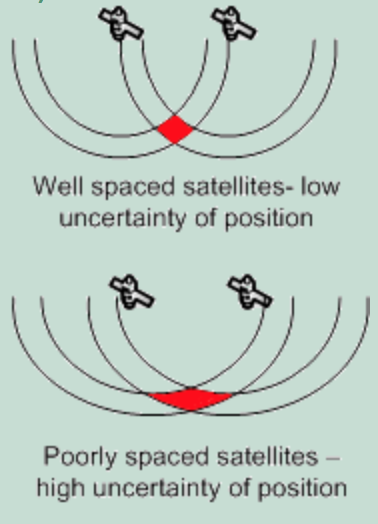
\includegraphics[width=0.4\textwidth]{sections/Conclusion/bunchedsat.png}
	\caption{Klumpede og spredte satelitter}
	\label{fig:bunchedsat}
\end{figure}

Kondisjonstallene og de maksimale posisjonsfeilene regnet i oppgave 4 og 5 er avhengige av satelittposisjonene, så derfor kan ikke disse betraktes som de største mulige verdiene for disse egenskapene. Derfor er egentlig disse tallene lave grenser for kondisjonstallet til GPS-problemet. 

\vspace{5mm}

Måten GPS kalkulerer posisjonen til brukeren er at man vet avstanden fra 3 forskjellige satelitter. Disse 3 avstandene møtes bare i 2 punkter, hvorav ett av disse lett kan utelukkes på grunn av at det ligger utenfor jordas overflate. Dette gjøres ved at hver satelitt sender sin tid til mottakeren, og mottakeren finner hvor langt unna denne satelitten er med å regne tidsforskjellen fra satelittens tid til mottakerens tid, og ganger dette med lyshastigheten. I teorien trenger vi da bare 3 satelitter for å fastsette en posisjon, men på grunn av at mottakerens klokke er relativt unøyaktig i forhold til satelitten, kan dette føre til at posisjonen blir feil med flere kilometer. Derfor trenger vi 4 satelitter for å fastsette den virkelige tiden d, og får derav 4 likninger med 4 ukjente. Her er det verdt å merke seg at hvis vi kunne målt tiden hos mottakeren 100\% nøyaktig, ville den siste satelitten vært unødvendig, og vi kunne funnet posisjonen nøyaktig med 3 satelitter. 

\vspace{5mm}

Andre feilkilder som bidrar til at GPS ikke er 100\% nøyaktig, er at lysfarten ikke er lik fra jordas overflate og opp til satelittene. Dette vil føre til at tiden vi regner med at det tar for signalet å komme frem blir litt unøyaktig, ettersom vi i utregningene har regnet med en konstant lyshastighet c. En annen feilkilde er at vi i denne oppgaven tar det for gitt at signalet fra satelittene går i en rett linje til mottakeren. I virkeligheten har man diverse obstruksjoner som gjør at signalet kan brytes i forskjellige retninger. Dette fører til at mottakeren mottar det samme signalet til forskjellige tider, noe som fører til enda en usikkerhet. Til slutt finnes det i virkeligheten diverse naturlige og menneskeskapte signaler som vil forstyrre signalet fra satelittene. I virkeligheten er alle disse problemene enten fjernet helt eller redusert, men dette er ikke gjort i vår oppgave. Derfor blir ikke våre posisjoner like nøyaktig som GPS er i virkeligheten. 
\newpage
% section konklusjon (end)

\newpage
\section{Referanseliste}
\begin{thebibliography}{9}
\bibitem{Boka}
  Sauer, Timothy. 
  \emph{Numerical Analysis, Second Edition}
  Pearson Education Limited 2014, Edinburgh Gate, Harlow, England And Associated Companies throughout the world

\bibitem{TheDeterminant}
  Yoichiro, Mori (2013).
  \emph{The Determinant} Tilgjengelig fra \url{http://math.umn.edu/~ymori/docs/teaching/spring13/ch5.pdf}  (Hentet: 14.04.15).

  \bibitem{Determinants}
  Mangahas, Johanna. \emph{Determinants} Tilgjengelig fra \url{http://www.math.brown.edu/~mangahas/det.pdf} (Hentet 16.04.15).
  
  \bibitem{Errors}
  Whitman College, \emph{Notes on error analysis} Tilgjengelig fra \url{http://people.whitman.edu/~hundledr/courses/M467F06/ConvAndError2.pdf} (Hentet 21.04.15).
  
  \bibitem{StrangBorre}
  Strang and Borre, Aalborg University
  \emph{Linear Algebra, Geodesy and GPS} Tilgjengelig fra \url{ftp://athena.fsv.cvut.cz/pub/mervart/StrangBorre.pdf} (Hentet 22.04.15).
  
  \bibitem{DGPS}
  Morag Chivers, Trimble 
  \emph{Differential GPS Explained} Tilgjengelig fra \url{http://www.esri.com/news/arcuser/0103/differential1of2.html} (Hentet 22.04.15).
  
\end{thebibliography}
%Hentet fra http://www.ntnu.no/viko/oppgave/harvardliste
%Webside
%Forfatter (�r) Tittel i kursiv. Tilgjengelig fra: URL (Hentet: dato).
%Fugelsnes, E. (2004) Oppvarmet st�v kan gi �kte helseplager. Tilgjengelig fra: http://www.forskning.no/Artikler/2004/mars/1079517069.32 (Hentet: 01. april 2004).
%Webside uten forfatter
%Tittel i kursiv (�r) Tilgjengelig fra: URL (Hentet: dato).


\section{Vedlegg} % (fold)
\label{sec:vedlegg}
Her vil du plassere alt som ikke er direkte relevant for rapporten, og som kun vil leses av et lite antall mennesker. Selv de fleste sensorer vil kanskje sjekke kun ett vedlegg for a se at det inneholder det du sier og at det er greit disponert. Hvis man utvikler programvare vil vanligvis utskrift av all kode ligge i vedlegg, mens utdrag fra denne legges inn i bilder eller figurer i teksten, der hvor dette er naturlig. Dette er ogsa stedet for matematisk bevis og liknende (det er forskjell pa matematiske bevis og matematiske teorier og omrader – det siste skal plasseres i teoridelen).
% section vedlegg (end)

\end{document}

